\begin{figure}[t]
\centering
    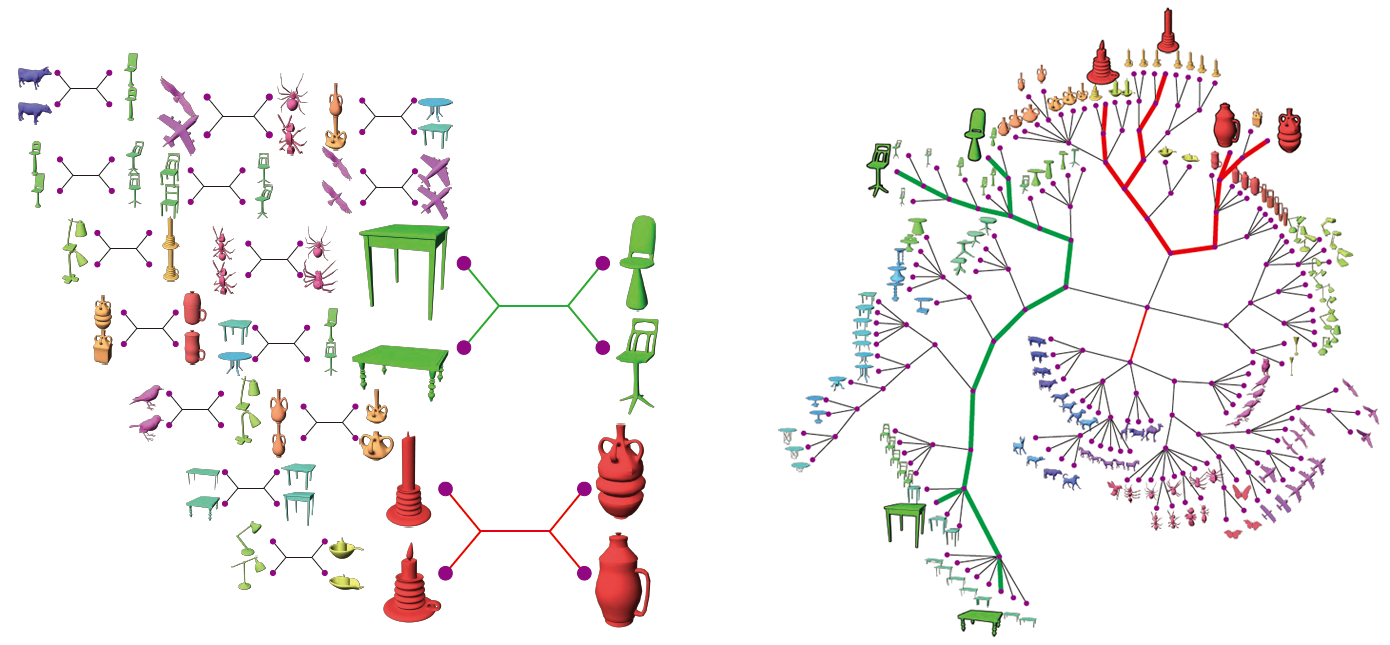
\includegraphics[width=1.0\columnwidth]{fig/img/huang_sig12_quartet}
    %\vspace{-0.4cm}
    \caption{Given a set of heterogeneous shapes, a reliable qualitative similarity is derived from quartets composed of two pairs of objects (left).
    Aggregating such qualitative information from many quartets computed across the whole set leads to a categorization tree as a hierarchical
    organization of the input shape collection (right).}
    \label{fig:huang_sig12_quartet}
\end{figure}

